\section{Scientific highlights}

\subsection{\nuc{7}{Be}\reac{p}{\gamma}\nuc{8}{B} (NABONA and DRS) }
The proton radiative capture on \nuc{7}{Be} ($T_{1/2} = 53.3$ days) is one of the most important reactions in nuclear astrophysics as it determines the number of the highest energy neutrinos emerging from a hydrogen burning star like our sun. As human science has now entered the precision phase in solar neutrino detection with real time detectors like SNO, Super-Kamiokande and Borexino, the error on the rates of the neutrino producing nuclear reaction in the hydrogen burning chains become the limiting factors in the interpretation of the measured neutrino fluxes. Our cross section information so far encompasses predominantly solid \nuc{7}{Be} targets of varying purity, complemented with data from Coulomb breakup experiments where the inverse reaction is measured. With claimed uncertainties below 5\% the measurements fall within a 20\% band suggesting that systematical uncertainties are present. In order to try an approach with different systematic uncertainties two attempts were made so far to measure this reaction using a radioactive beam and recoil separator detection. In both cases the radioactive material was not produced on-line but sent from an off-site producer, chemically treated and concentrated before being used in a standard sputter source \cite{gial00}. The first attempt at this reaction was performed with the NABONA recoil separator in Naples. The accelerator provided an 8 MeV \nuc{7}{Be} ion beam in the $4^+$ charge state of up to 30 epA varying over several days. This intensity was unfortunately not sufficient to make a statistically significant measurement yielding only 13 recoil events identified as \nuc{8}{B} by the $\Delta{}E-E$ IC in the focal plane (Fig.\ \ref{fig:gialanella00_fig2}: Fig. 2 from \cite{gial00}).
\begin{figure}
\begin{center}
\resizebox{0.95\columnwidth}{!}{
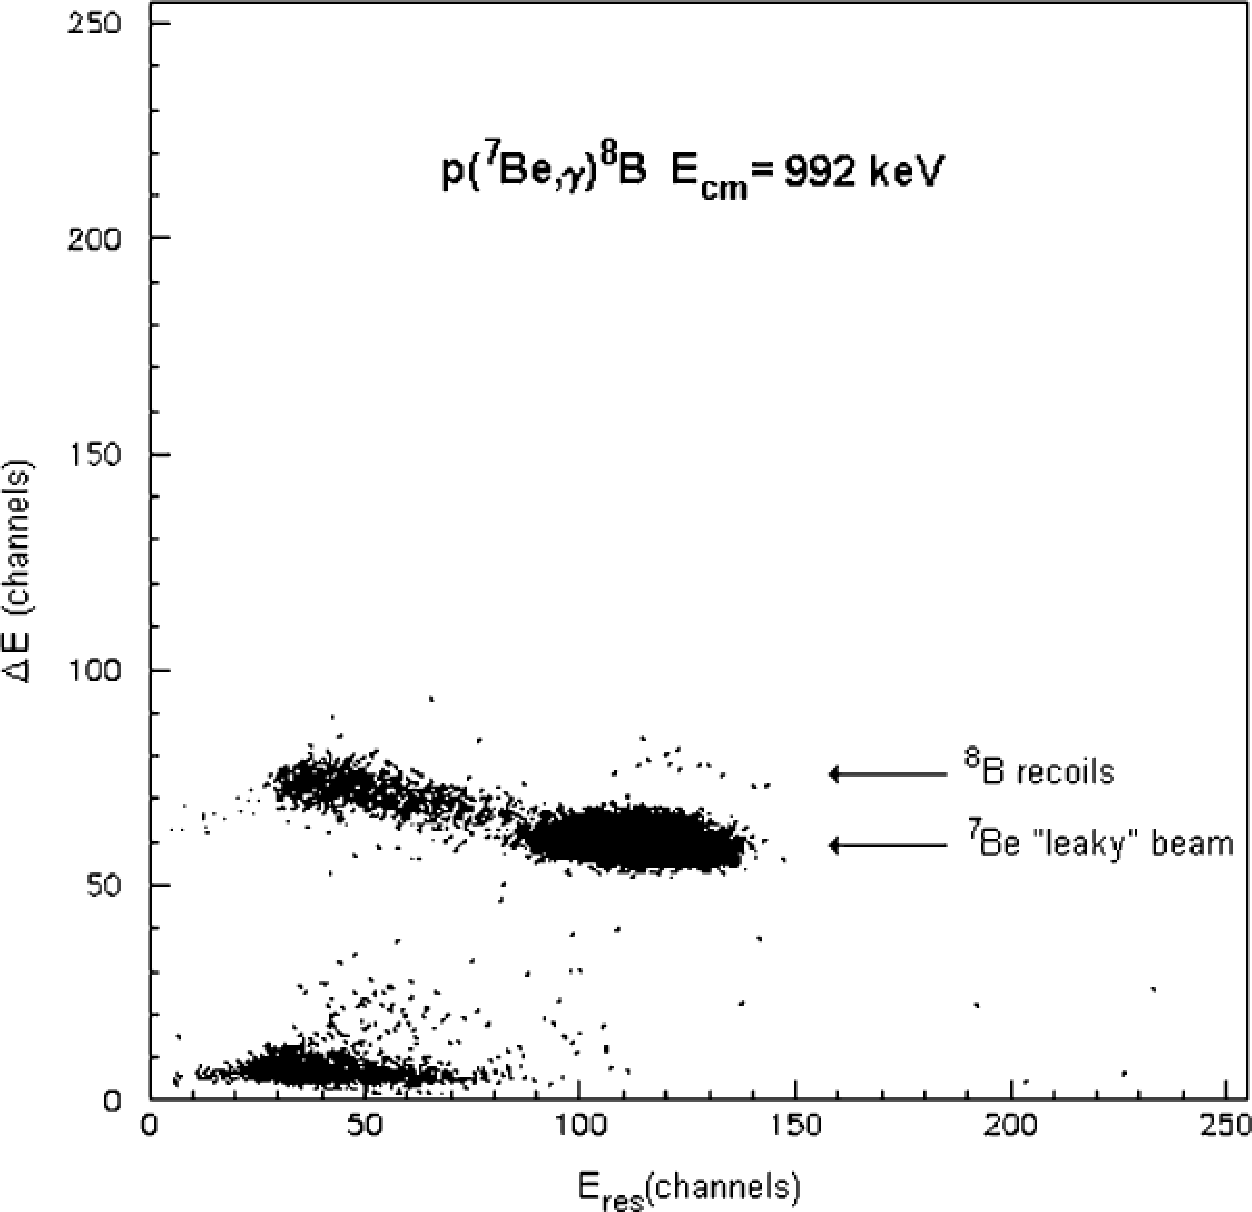
\includegraphics{Gialanella00_Fig2_DeltaE-E}
}
\caption{Two dimensional density plot of the $\Delta{}E-E$ telescope with the recoil separator tuned to the \nuc{8}{B}$^{5+}$ nuclides from $p$(\nuc{7}{Be},$\gamma$)\nuc{8}{B} reaction. The observed structures are identified. Taken from \cite{gial00}.}
\label{fig:gialanella00_fig2}
\end{center}
\end{figure}
The beam intensity produced in Naples already required performance of the radiochemical procedures with activities of the order of 10 -- 20 GBq and it was not deemed practical to increase on these. Therefore, this reaction was not pursued further at this accelerator facility. Several years later, the HRIBF facility was able to increase ion source efficiency and accelerator transmission but was only capable to handle a reduced activity in the radiochemistry. Therefore, they achieved a similar \nuc{7}{Be} ion beam intensity, this time stable over several days, but again only an insufficient number of recoils (Fig.\ \ref{fig:bardayan09_fig4}: Fig. 4 of \cite{bard09}).
\begin{figure}
\begin{center}
\resizebox{0.98\columnwidth}{!}{
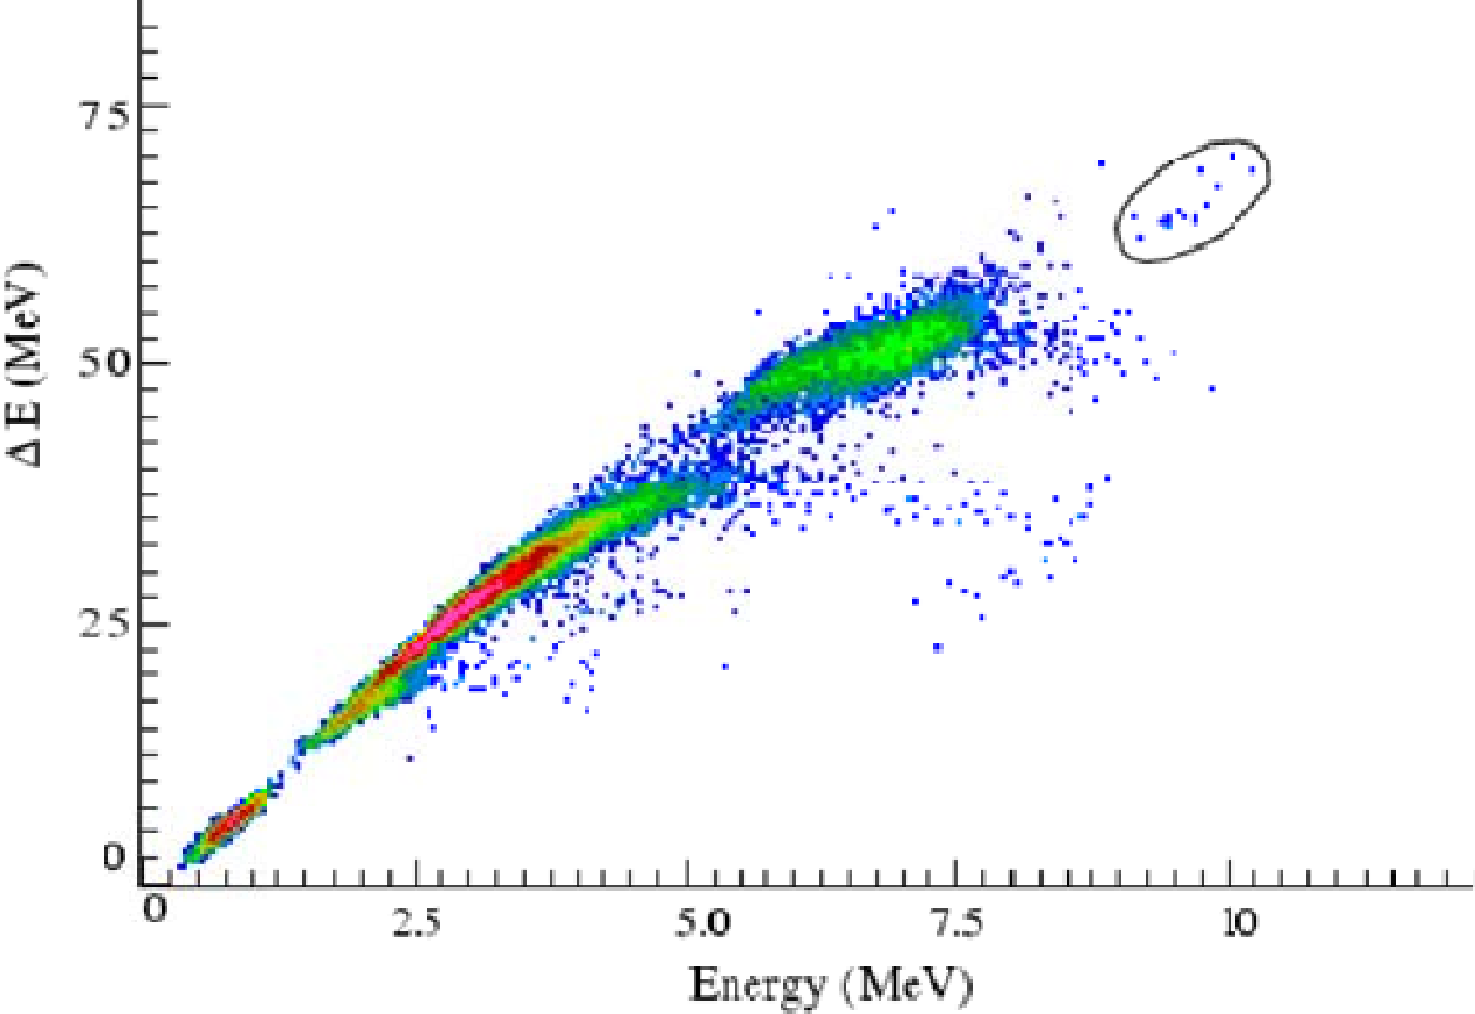
\includegraphics{Bardayan09_Fig4_Be7pg_DeltaE-E.pdf}
}
\caption{An ion counter $\Delta{}E$ vs. $E$ spectrum obtained for the \nuc{1}{H}(\nuc{7}{Be},$\gamma$)\nuc{8}{B} reaction. Events from \nuc{8}{B} recoils are circled. Taken from \cite{bard09}.}
\label{fig:bardayan09_fig4}
\end{center}
\end{figure}%
Significant to mention is that both attempts did not need $\gamma$ detection but it was sufficient to use nuclear charge identification with an IC at the focal plane. Although both experiments were performed at the same beam energy with similar gas target configurations, the leaky $^7$Be beam signature in the equally similar focal plane detectors appears very different probably due to the differences in separator configuration. It should be noted that in both attempts methods were developed to achieve the required uncertainties in {\it e.g.} beam normalization and solid angle determination. However, as it became clear that the statistics to return a relevant data point could not reached, many of these ancillary measurements were not followed through on. 


\subsection{\nuc{21}{Na}\reac{p}{\gamma}\nuc{22}{Mg} (DRAGON)}
The \nuc{21}{Na}\reac{p}{\gamma}\nuc{22}{Mg} reaction was the first to be measured with radioactive beam at the DRAGON facility, and the high intensity $^{21}$Na beam was one of the first to be accelerated at TRIUMF-ISAC, being a relatively easy ISOL beam to produce because of the high surface ionization efficiency of sodium using high-power silicon-carbide targets at ISAC, which are capable of producing pure $^{21}$Na beams on the order of $1 \times 10^{10}$ s$^{-1}$. 
The \nuc{21}{Na}\reac{p}{\gamma}\nuc{22}{Mg} reaction itself is a potential bypass to the $\beta^{+}$ decay of $^{21}$Na in the Ne-Na-Mg cycle that occurs in O-Ne-Mg novae. When \nuc{21}{Na}\reac{p}{\gamma}\nuc{22}{Mg} becomes faster than the decay, $^{22}$Na is made sooner. If this happens at times when the expanding nova envelope is hotter, $^{22}$Na can then be destroyed more quickly via proton capture. The net effect is that the faster \nuc{21}{Na}\reac{p}{\gamma}\nuc{22}{Mg} is at peak nova temperatures, the less $^{22}$Na survives in the ejecta. Since $^{22}$Na is one of the most promising candidates for direct observation from novae, it is important that the \nuc{21}{Na}\reac{p}{\gamma}\nuc{22}{Mg} reaction is known to sufficient precision to remove the nuclear physics uncertainty from $^{22}$Na ejected yield predictions.  

The \nuc{21}{Na}\reac{p}{\gamma}\nuc{22}{Mg} reaction at nova temperatures is dominated by several strong resonances corresponding to states in $^{22}$Mg. These states were identified previous to the DRAGON experiment in several indirect studies such as $^{24}$Mg(p,t)$^{22}$Mg \cite{bat01,mic02} and $^{25}$Mg($^{3}$He,$^{6}$He)$^{22}$Mg \cite{cag02}, as well as $^{12}$C($^{16}$O,$^{6}$He)$^{22}$Mg \cite{che01}, and $^{20}$Ne($^{3}$He,n$\gamma$)$^{22}$Mg \cite{rol72}. 
This information identified the likely candidates for strong resonances that would contribute to \nuc{21}{Na}\reac{p}{\gamma}\nuc{22}{Mg}, and thus all resonance strengths were able to be measured by DRAGON over a 2 year period, including those at higher energies more applicable to X-ray bursts. Subsequent other studies \cite{rui05,sew05} were able to make sense of the $^{22}$Mg level scheme and suggest that no resonances had been missed in the study, making this reaction the most completely studied RIB radiative capture process for astrophysics.  

A precision measurement of the dominant resonance in \nuc{21}{Na}\reac{p}{\gamma}\nuc{22}{Mg}, that at E$_{c.m.}$=205.7 keV, found the strength to be somewhat larger than expected from previous 
estimates \cite{jos99}. The result is that the reaction rate is stronger at typical O-Ne-Mg nova temperatures, and results in less $^{22}$Na being ejected, and thus a reduction in the observable 1.275 MeV $\gamma$-ray flux when compared with the old value of the rate. In addition, the energy of the resonance was measured with high precision at DRAGON using the thick target scan method, resulting in E$_{c.m.}$=205.7$\pm$0.5 keV. Combining this with precision values of the excitation energy, it was determined that the mass excess of $^{22}$Mg in the literature was incorrect by almost 7 keV, a fact that was subsequently corroborated in a new evaluation of the $^{22}$Mg mass excess \cite{har03}.  

\subsection{\nuc{26g}{Al}\reac{p}{\gamma}\nuc{27}{Si} (DRAGON)}
The \nuc{26g}{Al}\reac{p}{\gamma}\nuc{27}{Si} reaction is of importance in understanding the origin of galactic $^{26}$Al [t$_{1/2}=(7.2\pm0.2)\times10^{5}$yr], which has been mapped via observation of its 1.809 MeV $\gamma$ ray using several space-based telescopes (such as COMPTEL and INTEGRAL) \cite{smi03,kno04,die95}. The contribution of O-Ne-Mg novae to this distribution was relatively uncertain due to uncertain natures of both the \nuc{25}{Al}\reac{p}{\gamma}\nuc{26}{Si} and \nuc{26g}{Al}\reac{p}{\gamma}\nuc{27}{Si} reactions, in particular a resonance at E$_{c.m.}$=184 keV in the latter, to which the ejected $^{26g}$Al yield is particularly sensitive. This resonance was measured \cite{rui06} at the DRAGON facility using an accelerated $^{26g}$Al beam of up to $5\times10^{9}$ s$^{-1}$. This is still, as far as the authors are aware, the highest post-accelerated RIB intensity achieved anywhere. This experiment posed several challenges: although the $^{26}$Al was ionized using a resonant laser system (after being produced in a high-power silicon carbide target at ISAC), a substantial component of $^{26}$Na (t$_{1/2}$=1.07 s) was present in the beam from surface ionization, enough to cause a high rate in the DRAGON BGO detector array from $^{26}$Na decay at the target entrance aperture. To combat this, DRAGON used  a mechanical IRIS upstream of the gas target to trim the small amount of beam halo that was causing the rate from the target aperture, effectively reducing rate in the BGO detectors (and thus lowering the randomly-coincident background level). In addition, around $1\times10^{6}$ s$^{-1}$ of the metastable state of $^{26m}$Al (t$_{1/2}$=6.35 s) was present in the beam. The rates of these beam contaminants were measured using some of the ancillary detectors mentioned in previous sections, the $^{26}$Na via the decay $\gamma$ ray at 1.809 MeV, measured with a HPGe detector, and the $^{26m}$Al using a `horn' to collect positrons leading to annihilation 511 keV $\gamma$ rays measured with two opposing NaI detectors. By providing feedback signals to the ISAC operators, tuning of the ISAC high resolution mass separator was able to reduce the rate in the BGO detectors from $^{26}$Na to almost zero. The metastable component could not be resolved because of its similarity in mass to the ground state. 
These experimental improvements enabled the measurement of the resonance, which remains the weakest resonance strength to have ever been measured in inverse kinematics using a RIB, at $\omega\gamma=35\pm7 \mu$eV. 
%The measurement of this strength enabled hydrodynamic calculations of an O-Ne-Mg WD nova of 1.25M$_{\odot}$ to be performed with increased confidence in the rate of the $^{26}$Al direct destruction mechanism, leading to a sustained conclusion that such novae are minor secondary contributors to the total galactic $^{26}$Al distribution. 

\subsection{\nuc{17}{F}\reac{p}{\gamma}\nuc{18}{Ne} (DRS) }
The measurement of the  \nuc{1}{H}(\nuc{17}{F},$\gamma$)\nuc{18}{Ne} reaction has been so far the only radiative capture experiment at the DRS using an online produced radioactive ion beam from the HRIBF. This reaction is an important pathway in the hot CNO cycles in novae and believed to provide a significant energy boost to x-ray bursts through the reaction sequence \nuc{14}{O}\reac{\alpha}{p}\nuc{17}{F}($p$,$\gamma$)\nuc{18}{Ne}\reac{\alpha}{p}\nuc{21}{Na}. In the experiment at ORNL a mixed \nuc{17}{F} beam was available (typically \nuc{17}{F} $\approx$ 35 -- 70\% of the total mixed with \nuc{17}{O}) which was focused through the windowless gas target containing 4 Torr of Hydrogen. The \nuc{17}{F} content was monitored using a sampling mechanism which periodically intercepted the beam after the gas target and measured the $\beta^+$-decay of the \nuc{17}{F} implanted in the sampling plate between two plastic scintillator detectors. Over the several days the experiment lasted beam currents in the $10^6$ 1/s were available. Again, at the DRS no measurement of the reaction $\gamma$-rays was attempted and the analysis fully relied on the nuclear charge separation in the $\Delta{}E-E$ ionization chamber. For this purpose extensive calibration measurements using the \nuc{17}{O}($p$,$\gamma$)\nuc{18}{F} as well as \nuc{17}{O}+\nuc{20}{Ne} elastic scattering were performed to identify the neon recoil signature in the instrument. The final ionization chamber spectrum (data was taken at 3 charge states in total) shows the two leaky beam components as well as a clear agglomeration of events in the expected area for \nuc{18}{Ne} recoils (Fig.\ \ref{fig:chipp09a_3}: Fig. 3 from \cite{chip09a}).
\begin{figure*}
\begin{center}
\resizebox{1.6\columnwidth}{!}{
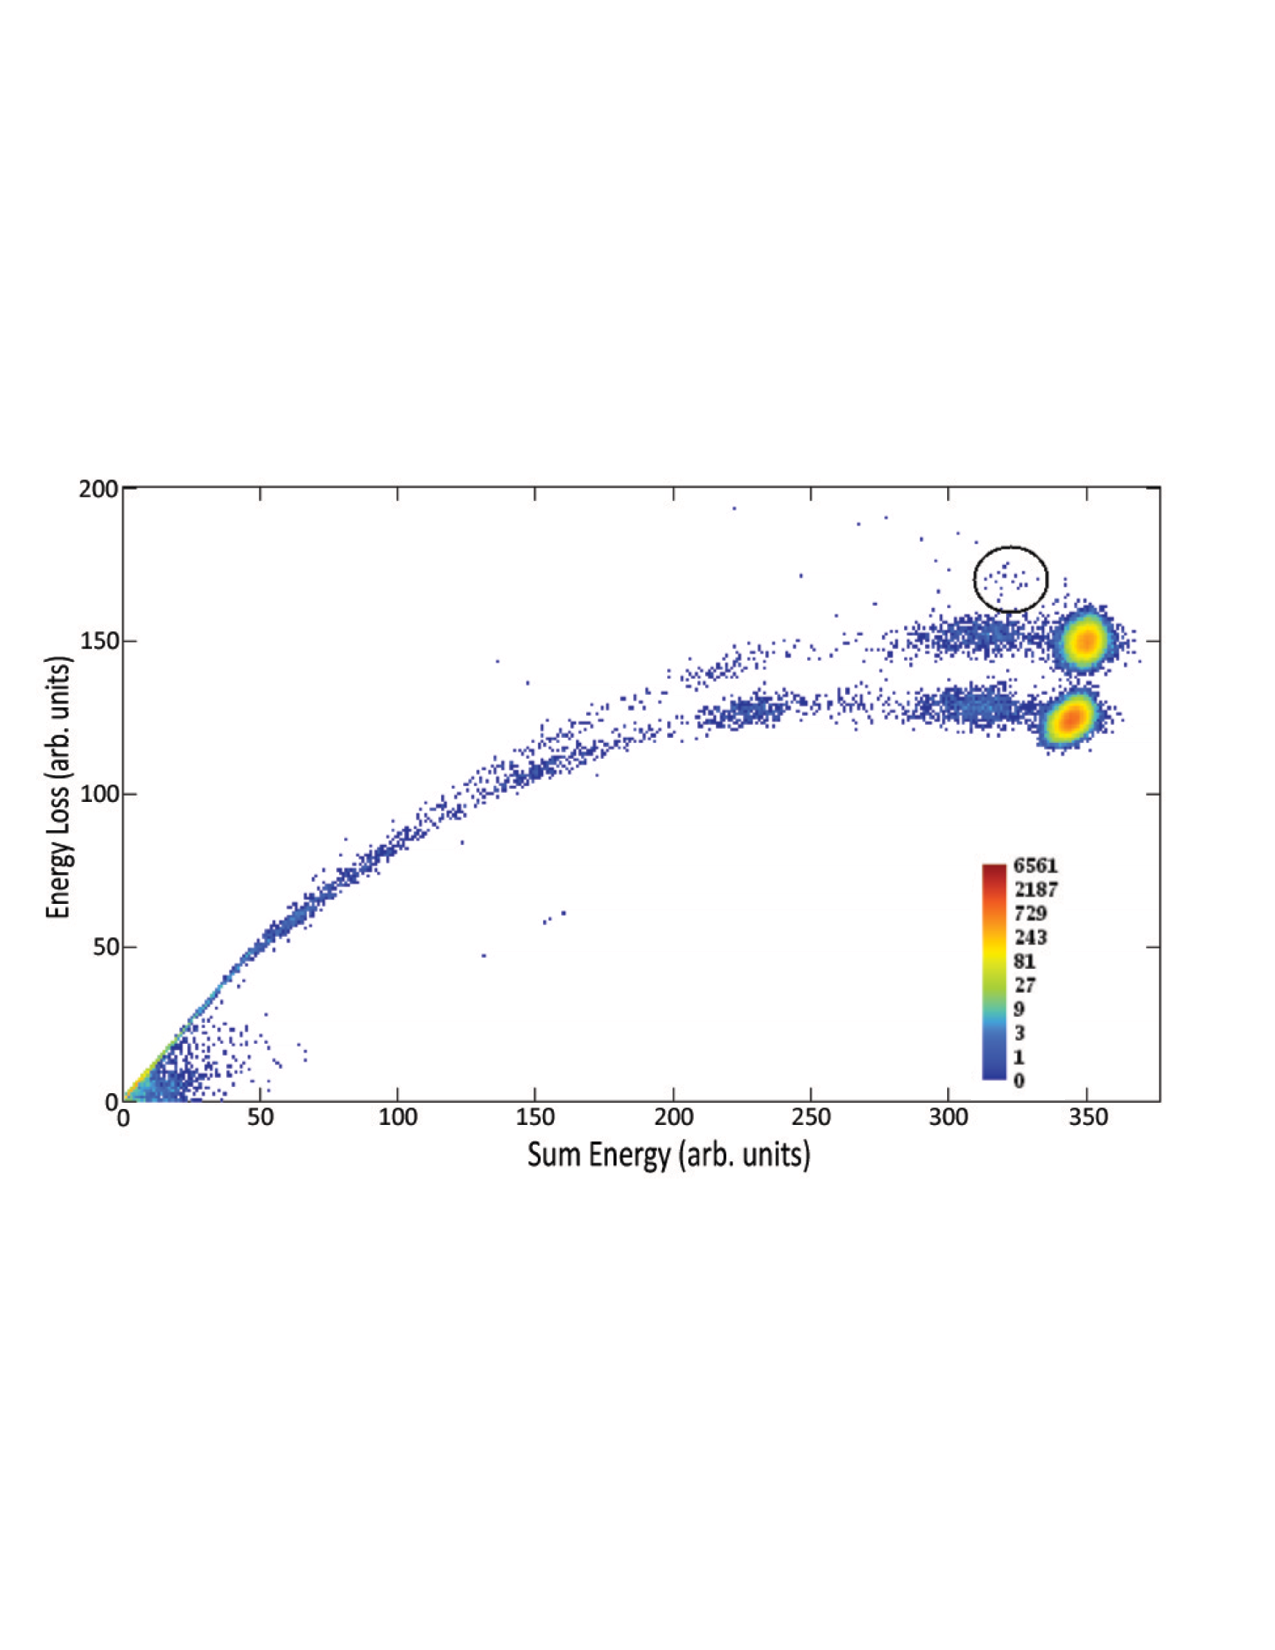
\includegraphics{chipps_fig06}
}
%\vspace{5cm}       % Give the correct figure height in cm
\caption{Energy loss versus total energy from the ionization chamber for the 599.8 keV resonance; \nuc{18}{Ne} recoils are indicated by the black circle. Taken from \cite{chip09a}.}
\label{fig:chipp09a_3}
\end{center}
\end{figure*}
Given the amount of background visible, this experiment, yielding an $\omega\gamma \approx 30 \unit{meV}$, was clearly showing the limits of the sensitivity of the DRS setup. Further improvements would be possible through the addition of a $\gamma$ array around the target to allow coincidence measurements and efforts to further suppress the leaky beam components transmitted to the focal plane.

\subsection{\nuc{23}{Mg}\reac{p}{\gamma}\nuc{24}{Al} (DRAGON)}
The \nuc{23}{Mg}\reac{p}{\gamma}\nuc{24}{Al} is another which affects the ejected abundance of $^{22}$Na (and to a lesser extent, $^{26g}$Al) in O-Ne-Mg novae \cite{ilia02}, though the large variation came mainly from the large uncertainty in the rate rather than the sensitivity of the $^{22}$Na yields to small variations in the rate. This large uncertainty stemmed mainly from the absence of direct measurements of the reaction and sparse indirect experimental information concerning the states in $^{24}$Al, mainly from the $^{24}$Mg($^{3}$He,t)$^{24}$Al reaction \cite{gre91,kub95,vis07,zeg08} and a $\gamma$-decay study using $^{10}$B($^{16}$O,2n$\gamma$)$^{24}$Al \cite{lot08}. 
The first direct measurement of the \nuc{23}{Mg}\reac{p}{\gamma}\nuc{24}{Al} reaction, in particular the $E_{R}=486$ keV dominant resonance at nova temperatures, was performed at the DRAGON facility \cite{eri10}. The $^{23}$Mg was produced using a high-power silicon carbide target at ISAC, and resonantly ionized using the ISAC laser ion source \cite{las09}. This resulted in an accelerated beam of mixed $^{23}$Na and $^{23}$Mg, with the peak $^{23}$Mg current of around $3\times10^{7}$ s$^{-1}$. The ratio $^{23}$Na:$^{23}$Mg was time-varying and ranged between (20:1 -- 1000:1). This presented the challenge of not only of determining the $^{23}$Mg integrated flux over the duration of the experiment, but also separating leaky A=23 beam components (both Na and Mg) from both $^{24}$Al and $^{24}$Mg recoils (the latter from \nuc{23}{Na}\reac{p}{\gamma}\nuc{24}{Mg}). This was done using a combination of local time-of-flight measurements by the DRAGON MCPs, $\Delta$E-E measurements in the multi-anode ionization detector, coincidence detection of particles with prompt $\gamma$-ray events in the BGO array, and separator time-of-flight. Figures \ref{fig:Mg23_tof_IC} and \ref{fig:Mg23_dE_E} show some example data for one of the DRAGON \nuc{23}{Mg}\reac{p}{\gamma}\nuc{24}{Al} runs. Checks were also performed by eliminating the $^{23}$Mg by switching off the laser ionization, to determine the extend of the $^{23}$Na-induced background.  
Due to an uncertainty in the true resonance energy, BGO hit pattern data indicated that the reactions were occurring upstream in the DRAGON extended gas target, rather than in the centre where expected given the adopted resonance energy of $E_{R}=473$ keV that was accepted before the experiment. Because it could not be certain that the reactions were occurring in plateau region of gas density in the target, a 2D probability distribution in the resonance strength ($\omega\gamma$) and resonance energy ($E_{R}$) variables could only be constructed, leading to extracted values of $E_{R}=485.7^{+1.3}_{1.8}$ keV and $\omega\gamma=38^{+21}_{-15}$ meV, with the central values and uncertainties taken as the medians and 16\% and 84\% quartiles of the 2D PDF. 
A re-evaluation of old measurements in the literature of the $^{24}$Al mass excess, combined with the $\gamma$-ray measurements of \cite{lot08} presented in the DRAGON work \cite{eri10}, also suggested that $E_{R}=480(6)$ keV (uncertainties at 1$\sigma$).     
A subsequent mass measurement \cite{wre10} of $^{24}$Al enabled a new determination of $E_{R}$, which was combined with the DRAGON results to result in adopted values of $E_{R}=484.3^{+1.3}_{1.7}$ keV and $\omega\gamma=26^{+15.4}_{-7.0}$ meV.
These results drastically reduce the uncertainty of the \nuc{23}{Mg}\reac{p}{\gamma}\nuc{24}{Al} rate to a level sufficient for nucleosynthetic calculations of O-Ne-Mg novae. The experiment represented an original challenge for a recoil separator when the RIB was embedded in a stable isobar component of much higher intensity. 

\begin{figure}
\begin{center}
\resizebox{1.0\columnwidth}{!}{
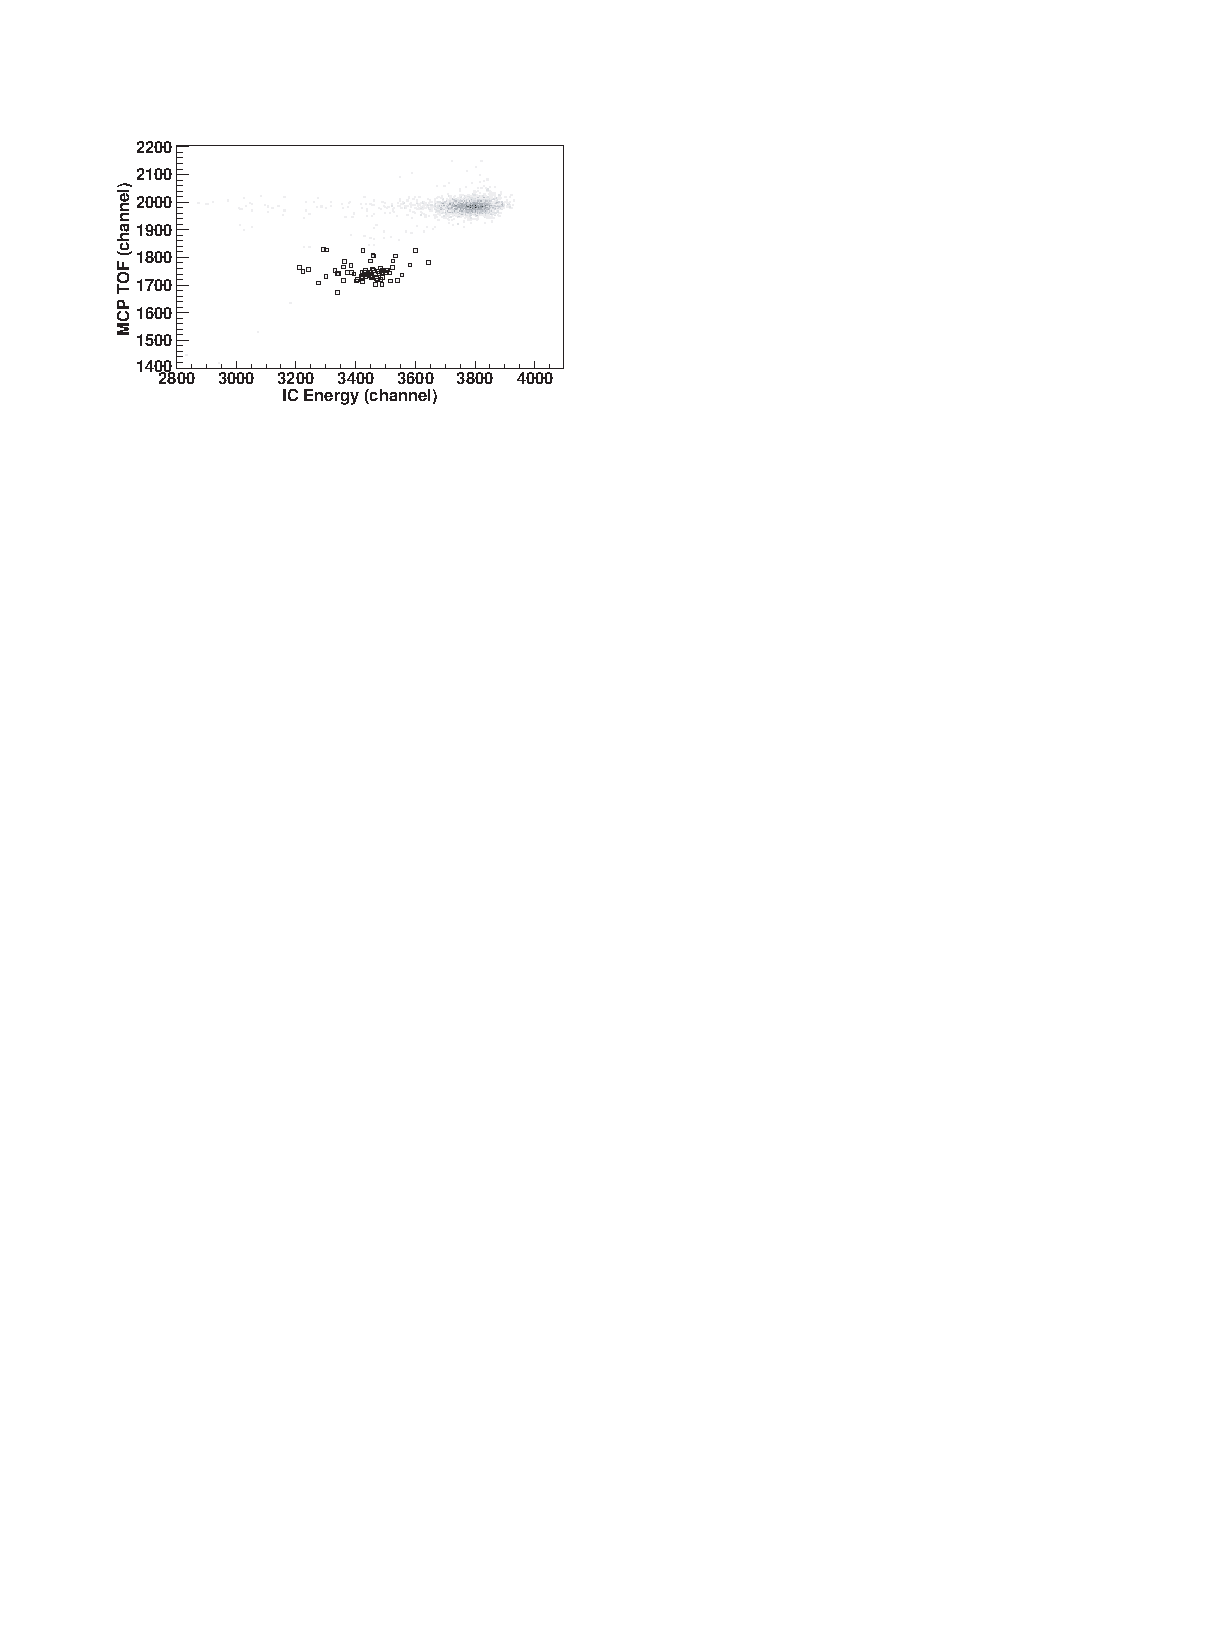
\includegraphics{Mg23_tof_IC}
}
\caption{Local time-of-flight vs. total detected energy for `singles' (not coincident with a prompt $\gamma$ ray) recoil events for the DRAGON \nuc{23}{Mg}\reac{p}{\gamma}\nuc{24}{Al} measurement. The grey density plot indicates all detected particles, while the open squares indicate A=24 recoils, clearly showing separation between `leaky' A=23 beam and A=24 recoils. Taken from \cite{eri10}.}
\label{fig:Mg23_tof_IC}
\end{center}
\end{figure}

\begin{figure}
\begin{center}
\resizebox{1.0\columnwidth}{!}{
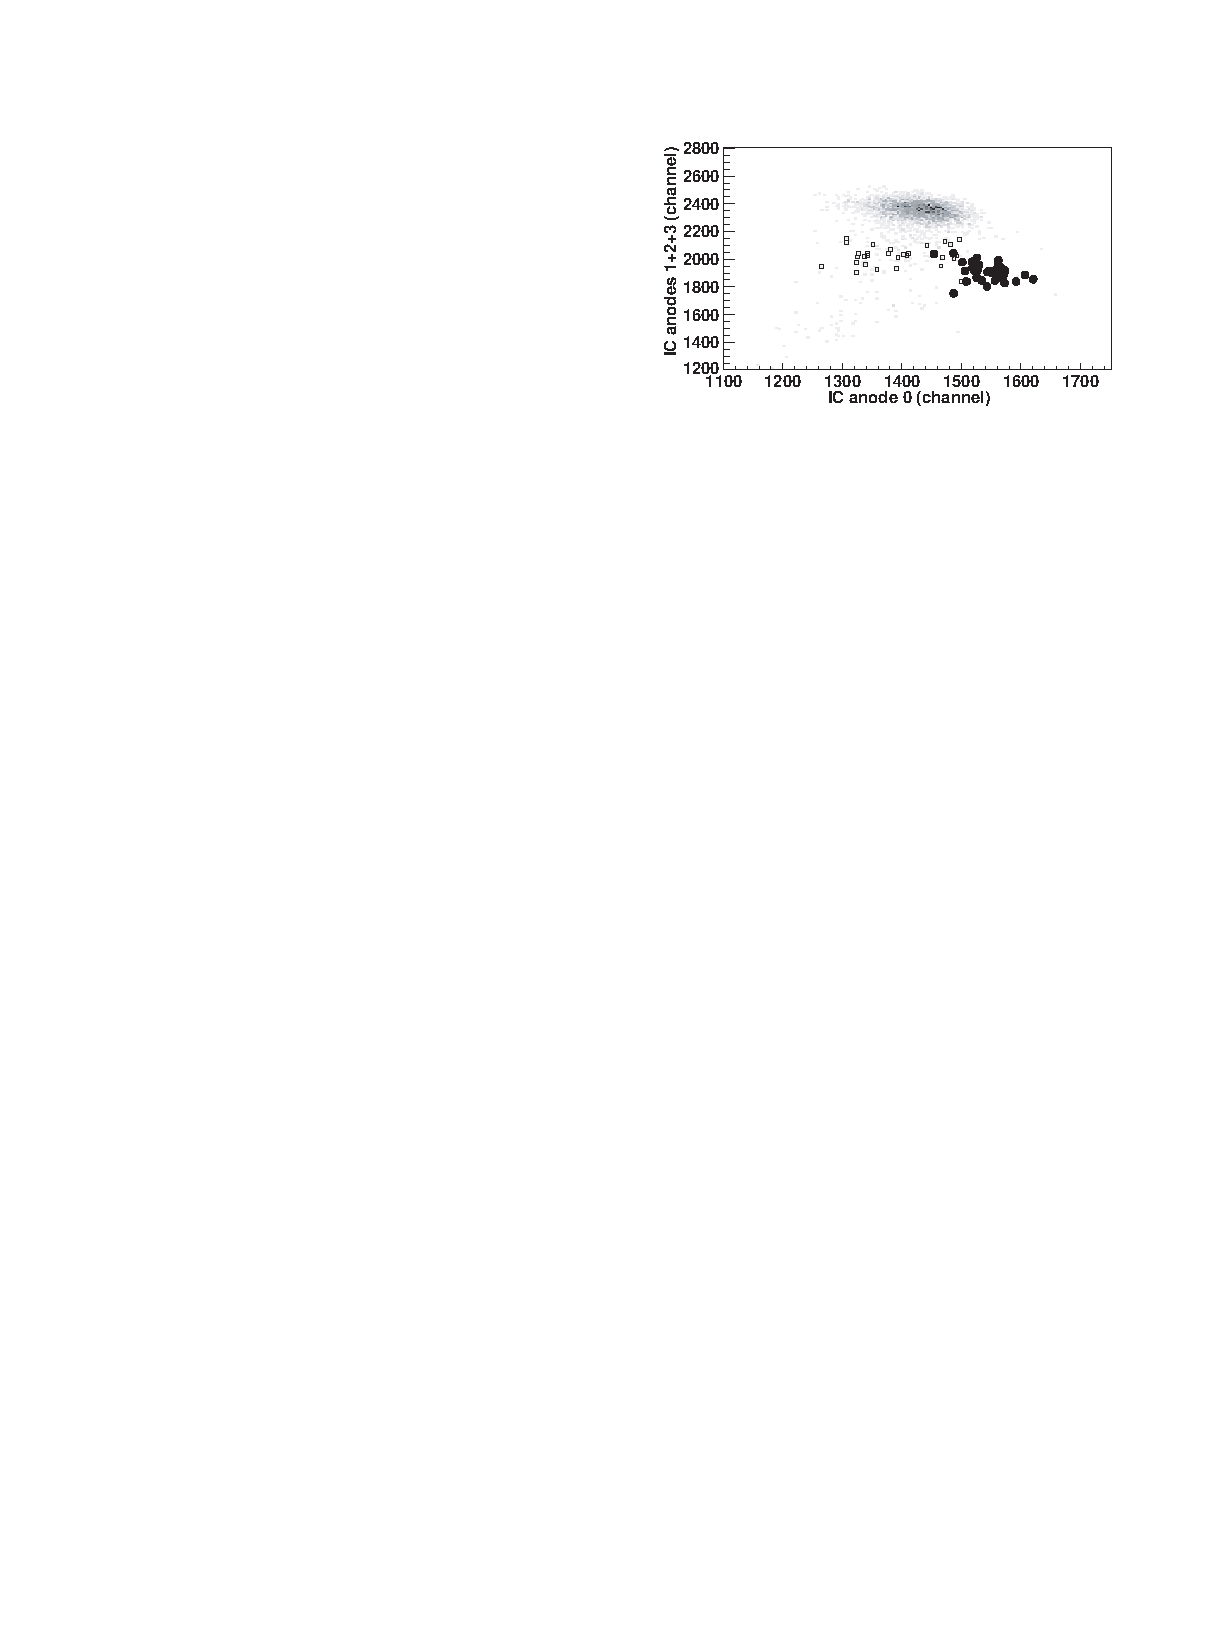
\includegraphics{Mg23_dE_E}
}
\caption{$\Delta$E vs. E for singles events in the DRAGON \nuc{23}{Mg}\reac{p}{\gamma}\nuc{24}{Al} measurement. The grey density plot indicates all detected particles. The open squares indicate all A=24 recoils, while the black circles indicate $^{24}$Al recoils. Taken from \cite{eri10}.}
\label{fig:Mg23_dE_E}
\end{center}
\end{figure}

\begin{figure}
\begin{center}
\resizebox{1.0\columnwidth}{!}{
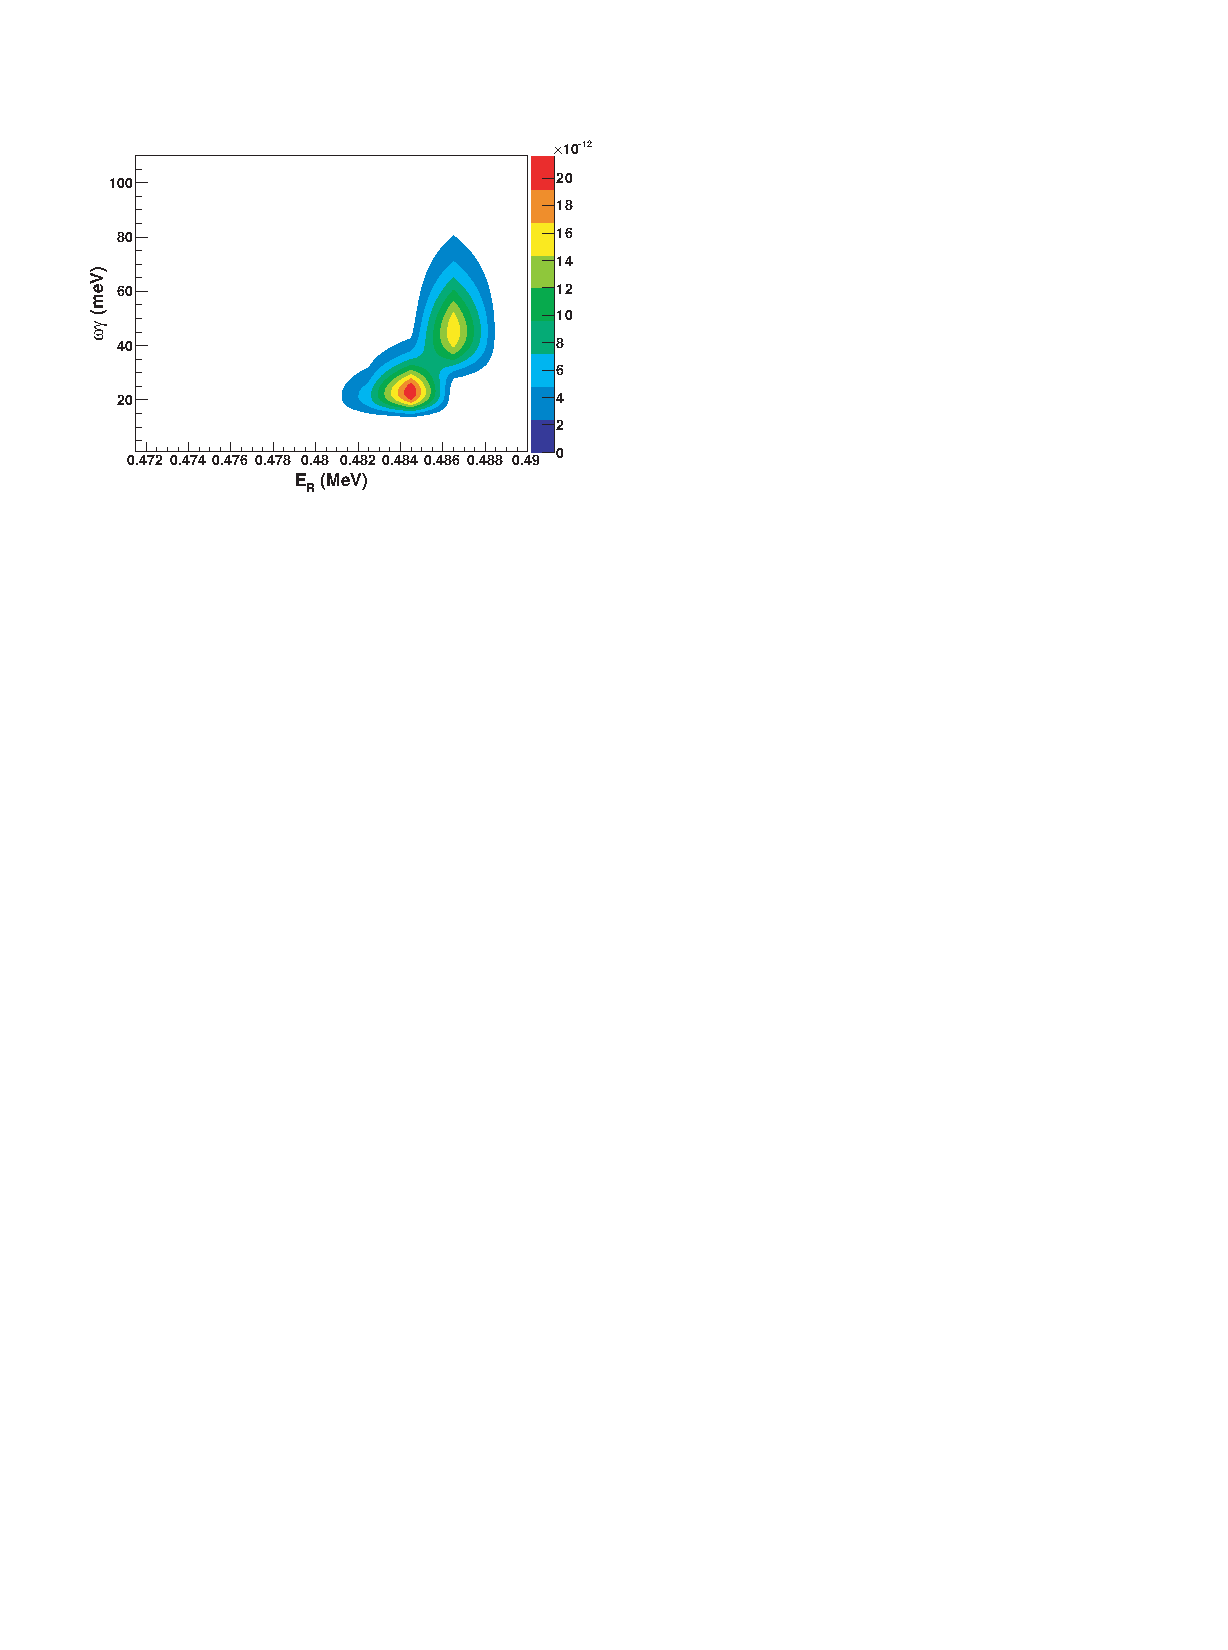
\includegraphics{Erikson_2010}
}
\caption{Probability contours for the determination of resonance strength, $\omega\gamma$, and resonance energy $E_{R}$, from the DRAGON measurement of \nuc{23}{Mg}\reac{p}{\gamma}\nuc{24}{Al}, taken from \cite{eri10}.}
\end{center}
\end{figure}